\documentclass{article}

\usepackage[style=numeric]{biblatex}
\usepackage{graphicx}

\renewcommand{\abstractname}{Resumen}
\renewcommand{\refname}{Bibliografía}
\setlength{\parskip}{1em}
\setlength{\parindent}{0em}
\usepackage{amsmath}

\begin{document}

\title{COMBINANDO VISIÓN ARTIFICIAL Y MODELOS DE LENGUAJE PARA INTERPRETACIÓN DE LENGUA DE SEÑAS CHILENA (LSCh)}

\author{Cristóbal Fajardo, Pablo Gaete, Rubén Torres \\ 
Profesor Guía: Juan Bekios}


\maketitle


\begin{abstract}

La escasez de intérpretes de Lengua de Señas Chilena (LSCh), especialmente en el ámbito de la salud, representa un desafío significativo para las personas sordas en Chile, dificultando el acceso a un tratamiento adecuado particularmente en el área de la salud mental. En este trabajo, se propone una solución digital que ofrece una alternativa accesible y de menor costo en comparación con los intérpretes profesionales. Nuestra propuesta combina la detección de puntos clave de las manos (hand landmark detection) con redes neuronales LSTM, complementadas por un modelo de lenguaje de gran escala (LLM) para lograr una mayor fluidez al transformar señas individuales en oraciones completa

El sistema ha demostrado una tasa de acierto del 92.5\% en el reconocimiento de palabras individuales y una similitud del 96.35\% comparado con las frases esperadas (utilizando la distancia de Levenshtein) en la traducción de frases completas. Además, utiliza una arquitectura cliente-servidor, que asegura escalabilidad y accesibilidad desde dispositivos con recursos limitados. A pesar de estos resultados prometedores, áreas como la ampliación del dataset y la reducción de latencia siguen siendo desafíos clave para el desarrollo futuro.

Esta solución digital no solo tiene el potencial de mejorar el acceso de las personas sordas en Chile a servicios críticos, sino que también abre nuevas oportunidades para la investigación y el desarrollo de tecnologías inclusivas en el ámbito de la comunicación asistida.

\end{abstract}

\section{Introducción}

\subsection{Descripción del problema}

En Chile, el II Estudio Nacional de la Discapacidad realizado por el Ministerio de Desarrollo Social y SENADIS en 2015 \cite{cita12}, el 16,7\% de la población presenta algún tipo de discapacidad, equivalente a 2.836.818 personas. De estas, el 3,6\% tiene dificultades auditivas, lo que representa aproximadamente 611.000 personas, de las cuales 180.000 padecen sordera total \cite{cita1}.

La escasez de intérpretes de Lengua de Señas genera una significativa exclusión de las personas sordas en nuestra sociedad, una situación particularmente evidente en el ámbito de la salud, uno de los pilares fundamentales para el bienestar humano.
En el ámbito de la salud mental, las personas sordas enfrentan una exclusión sistemática debido a la falta de comunicación efectiva con los profesionales, lo que incrementa los riesgos de exclusión social y dificulta su bienestar. Esta problemática resalta la necesidad urgente de soluciones tecnológicas que puedan abordar estas brechas de accesibilidad.

\subsection{Hipótesis de trabajo}

La implementación de un modelo de interpretación del Lenguaje de Señas Chileno (LSCh)
utilizando detección de manos con landmarks y redes neuronales LSTM, combinado con un
modelo de lenguaje (LLM) puede alcanzar una tasa de acierto mayor al 90\%, con un costo menor y una disponibilidad mayor que un intérprete humano.

\subsection{Objetivos}

\subsubsection{General}

Diseñar e implementar un sistema automatizado que interprete LSCh mediante visión artificial y procesamiento de lenguaje natural, para mejorar el acceso a servicios de salud por parte de personas sordas.


\subsubsection{Específicos}

\begin{enumerate}
    \item Investigar tecnologías avanzadas aplicadas al reconocimiento de lenguas de señas, incluyendo visión artificial y modelos de lenguaje.
    \item Implementar un modelo que integre MediaPipe para la detección de landmarks, LSTM para el análisis secuencial y LLM para la generación de traducciones coherentes.
    \item Evaluar la efectividad del sistema mediante métricas como precisión, similitud textual y latencia.
\end{enumerate}


\section{Estado del arte}

\subsection{Discusión Bibliográfica}

El reconocimiento de la Lengua de Señas Chilena (LSCh) ha sido un desafío técnico y social abordado en diversas investigaciones. Los primeros enfoques, como los modelos basados en Support Vector Machines (SVM), que corresponden a un conjunto de algoritmos de aprendizaje estadístico supervisado pertenecientes a la familia de los clasificadores lineales desarrollados por Vladimir Vapnik en torno al año 1995. Una SVM construye un hiperplano en un espacio de dimensionalidad muy alta y separa de forma óptima los puntos de una clase de la de otra. En el concepto de “separación óptima” es donde reside la característica fundamental de las SVM, se busca el hiperplano que tenga la máxima distancia (margen) con los puntos que estén más cerca de él mismo. Entre sus aplicaciones se encuentra el reconocimiento de email spam, escritura a mano y clasificación de imágenes.

Su implementación logró altos niveles de aciertos en ambientes controlados, alcanzando un 100\% en alfabetos visuales estáticos. Sin embargo, su desempeño disminuye significativamente en entornos no controlados, con aciertos de hasta un 80\% \cite{cita3}.

Este enfoque tiene algunas ventajas, como el uso eficiente de memoria, lo cual permite ser ejecutado en un dispositivo móvil Android. Sin embargo su principal limitación es que sólo puede identificar gestos estáticos, pero no secuencias de gestos, las cuales son necesarias para expresar muchos conceptos y oraciones \cite{cita4}. Otra limitación consiste en la falta de flexibilidad para funcionar bien en condiciones no ideales, por ejemplo, cuando la iluminación no es la más óptima.

Un enfoque más robusto es el modelo YOLO-v9e (You Only Look Once), una red neuronal convolucional diseñada específicamente para la detección de objetos en tiempo real. Este modelo, aplicado a la identificación de gestos que representan caracteres individuales del alfabeto, ha demostrado ser altamente efectivo  en conjuntos de datos de la Lengua de Señas Norteamericana (ASL) \cite{cita5}. YOLO-v9e, optimizada para estos escenarios, reportó una precisión del 96.83\%, un recall del 92.96\%, y un mAP@0.5 del 97.84\%, validando su capacidad para reconocer gestos con alta precisión en aplicaciones prácticas \cite{cita11} Sin embargo, éste presenta limitaciones para procesar secuencias, además requiere un gran volumen de datos etiquetados con precisión para cada gesto. En cual no está disponible en el caso de la LSCh. 

Ambos acercamientos tienen en común su factibilidad de ejecución en un dispositivo móvil, para permitir la portabilidad. Esta limitación la podemos superar al utilizar una arquitectura cliente-servidor que permita ejecutar el modelo de detección de las señas en un servidor con mayor capacidad computacional, y visualizar el resultado en un dispositivo móvil a través de una conexión a internet

Un avance importante en la interpretación de gestos secuenciales lo representan las redes convolucionales tridimensionales (3D-CNN) han mostrado ser capaces de procesar gestos secuenciales al modelar características espacio-temporales. Estas redes ofrecen una alta precisión para interpretar secuencias complejas, pero requieren altos recursos computacionales y grandes datasets etiquetados, lo que las hace menos viables para aplicaciones en lenguas de señas con recursos limitados \cite{cita9}.

Una forma eficiente de simplificar los datos de entrada del modelo es mediante la utilización de un sistema de landmarks, que sintetiza la información relevante en una serie de puntos clave, como las articulaciones y las puntas de los dedos. Estos landmarks actúan como una representación estructurada y compacta de los gestos, eliminando información redundante y preservando las características esenciales del movimiento. Este enfoque no solo optimiza el procesamiento de datos al reducir la complejidad del modelo, sino que también mejora la precisión en la identificación de gestos al proporcionar un conjunto consistente de referencias visuales que representan los movimientos de las manos de manera precisa \cite{cita6}.

Una vez superado el reto de identificar secuencias de gestos, permanece el reto de traducir al castellano de forma fluida y coherente. Un acercamiento que puede ser beneficioso en esta etapa, es la integración de un LLM. 

Los Modelos de Lenguaje de Gran Escala permiten interpretar variaciones en las señas dentro del contexto de frases completas, ofreciendo traducciones más precisas y coherentes que trascienden la mera clasificación de gestos individuales. El método SignLLM, basado en este enfoque, fue evaluado en los conjuntos de datos PHOENIX-2014T (lengua de señas alemana) y CSL-Daily (lengua de señas china), logrando resultados destacados. En PHOENIX-2014T, el modelo alcanzó una puntuación BLEU-4 de 25.25 en el conjunto de validación y 23.40 en el de prueba, mientras que en CSL-Daily obtuvo 12.23 y 15.75, respectivamente. Además, las puntuaciones ROUGE, que evalúan la recuperación del contenido clave, fueron de 47.23 (validación) y 44.49 (prueba) en PHOENIX-2014T, y de 39.18 (validación) y 39.91 (prueba) en CSL-Daily. Estas métricas demuestran que SignLLM logra mantener un equilibrio entre la precisión gramatical y la coherencia semántica, destacando su efectividad en comparación con otros métodos gloss-free que no utilizan glosas \cite{cita10}.


\subsection{Marco Teórico}

El marco teórico aborda las tecnologías clave que sustentan la interpretación automatizada de la Lengua de Señas Chilena (LSCh), incluyendo MediaPipe, redes LSTM, modelos de lenguaje natural (LLM), métricas de evaluación y una arquitectura cliente-servidor, que veremos a continuación, fundamentales para garantizar la precisión y eficiencia del sistema.

\subsubsection{MediaPipe y Procesamiento de Gestos}

MediaPipe es una herramienta de visión artificial que permite la detección en tiempo real de landmarks o puntos clave en las manos, como articulaciones y puntas de los dedos. Su diseño eficiente lo hace adecuado para dispositivos con recursos computacionales limitados, proporcionando datos estructurados que facilitan el análisis de gestos. 

\subsubsection{Procesamiento Secuencial: Redes LSTM}

Las redes LSTM (Long Short-Term Memory) son una variante de redes neuronales recurrentes diseñadas para modelar secuencias temporales y resolver problemas de aprendizaje a largo plazo. Utilizan tres puertas: olvido, entrada y salida, para controlar el flujo de información, permitiendo conservar información relevante y descartar datos innecesarios.

\subsubsection{Categorical Crossentropy}

La Categorical Crossentropy es una función de pérdida ampliamente utilizada en tareas de clasificación multiclase para medir la discrepancia entre la distribución predicha por un modelo (q(x)) y la distribución real (p(x)). Matemáticamente, se define como

\[
H(p,q) = - \sum_{x \in X} p(x) \log(q(x))
\]

\subsubsection{Adam (Adaptive Moment Estimation)}

Algoritmo de optimización que ajusta dinámicamente las tasas de aprendizaje utilizando promedios móviles de gradientes y sus cuadrados para mejorar la eficiencia del entrenamiento.

\subsubsection{Early Stopping}

Early Stopping es una técnica de regularización que monitorea el rendimiento de un modelo en un conjunto de validación durante el entrenamiento. Su objetivo es identificar el momento óptimo para detener el entrenamiento antes de que el modelo comience a sobre ajustarse a los datos de entrenamiento. 

\subsubsection{Modelos de Lenguaje Natural: LLM}

Los modelos de lenguaje de gran escala son sistemas entrenados en grandes corpus textuales para generar texto coherente y contextualizado. Estos modelos incorporan el contexto semántico de las palabras, lo que les permite producir traducciones fluidas y adaptadas a estructuras gramaticales complejas.

\subsubsection{Métricas de Evaluación}

En este proyecto, se emplearon tres métricas clave: la precisión (accuracy), que mide el porcentaje de predicciones correctas realizadas por el modelo; la función de pérdida categorical crossentropy, utilizada para evaluar la diferencia entre las distribuciones predicha y real en problemas de clasificación multiclase; y la distancia de Levenshtein, que calcula la similitud entre cadenas de texto al medir las transformaciones necesarias, como inserciones, eliminaciones o sustituciones, para convertir una cadena en otra. 

\subsubsection{Arquitectura Cliente-Servidor}

La arquitectura cliente-servidor es un modelo de diseño computacional que distribuye tareas entre un cliente (dispositivo del usuario) y un servidor centralizado. El cliente captura y envía datos al servidor, que los procesa utilizando modelos de inteligencia artificial y devuelve los resultados. Este diseño garantiza la escalabilidad y optimiza los recursos, permitiendo que el cliente realice operaciones ligeras mientras el servidor asume la carga computacional más intensiva.

\subsubsection{Arquitectura de YOLOv9}

YOLOv9 está optimizado para la detección de objetos en tiempo real mediante tres componentes clave: Backbone, que extrae características iniciales; Neck, que refina estas características para detección multi-escala; y Head, que predice cajas delimitadoras y probabilidades de clase para objetos de distintos tamaños.

Un elemento crucial es la fórmula de Confidence Score, que evalúa la calidad de las predicciones:

\[
\text{Confidence (C)} = P(\text{Object}) \times \text{IoU}_{\text{truth, pred}}
\]

Aquí, P(Object) representa la probabilidad de que haya un objeto en la caja predicha, mientras que IoUtruth mide la superposición entre la caja predicha y la caja verdadera.

\subsubsection{Arquitectura de SVM}

Las Máquinas de Soporte Vectorial (SVM) son modelos matemáticos utilizados en el aprendizaje automático para resolver problemas de clasificación, regresión y detección de anomalías. Basadas en principios geométricos y matemáticos robustos, las SVM se destacan por su capacidad para encontrar soluciones óptimas incluso en escenarios complejos y de alta dimensionalidad.  Su funcionamiento se organiza en etapas bien definidas que forman una especie de "flujo de arquitectura:

Figura 6. Arquitectura de Flujo del SVM
El objetivo de la SVM es encontrar el hiperplano que maximiza el margen, formulado como un problema de optimización.


\section{Modelo Propuesto: LSTM + Hand landmarker + LLM}

En esta sección se describe el modelo a utilizar para probar la hipótesis. A diferencia de los modelos SVG o YOLO, discutidos en el capítulo 2.1, la red LSTM puede capturar datos históricos de la secuencia de imágenes para poder interpretar señas y gestos de manera dinámica. Para el entrenamiento, se utilizarán datos de hand landmarks derivados del conjunto de datos original, de esta manera se descarta parte del ruido y se sintetiza información relevante.

Utilizando este mecanismo se pueden identificar gestos que corresponden a palabras o frases individuales. Al agrupar listas de palabras que forman una oración, el siguiente paso consiste en usarlas como entrada al LLM gpt-3.5-turbo, junto con un prompt que permita obtener una frase con la fluidez propia del lenguaje hablado.

\subsection{Arquitectura del sistema}

La arquitectura propuesta está compuesta por tres componentes principales. El primero, una capa de MediaPipe hand landmarker, para obtener la lista de coordenadas de los puntos clave para cada mano.

El segundo componente es una red LSTM, que combina capas bidireccionales LSTM y densas para procesar datos secuenciales. La primera capa LSTM bidireccional captura patrones temporales en ambas direcciones y devuelve secuencias completas para la siguiente capa. La segunda LSTM bidireccional resume la información en una representación compacta. Luego, una capa densa con 128 neuronas y activación ReLU permite aprender relaciones no lineales, seguida de un Dropout del 50% para evitar sobreajuste. Finalmente, una capa densa con activación softmax produce probabilidades para las clases objetivo.

El tercer componente consiste en utilizar gpt-3.5-turbo, para derivar oraciones fluidas, dada una lista de palabras, y el prompt “Convierte la siguiente secuencia de palabras de lengua de señas chilena a una frase en español coherente”

\begin{figure}[!hbtp]
    \centering
    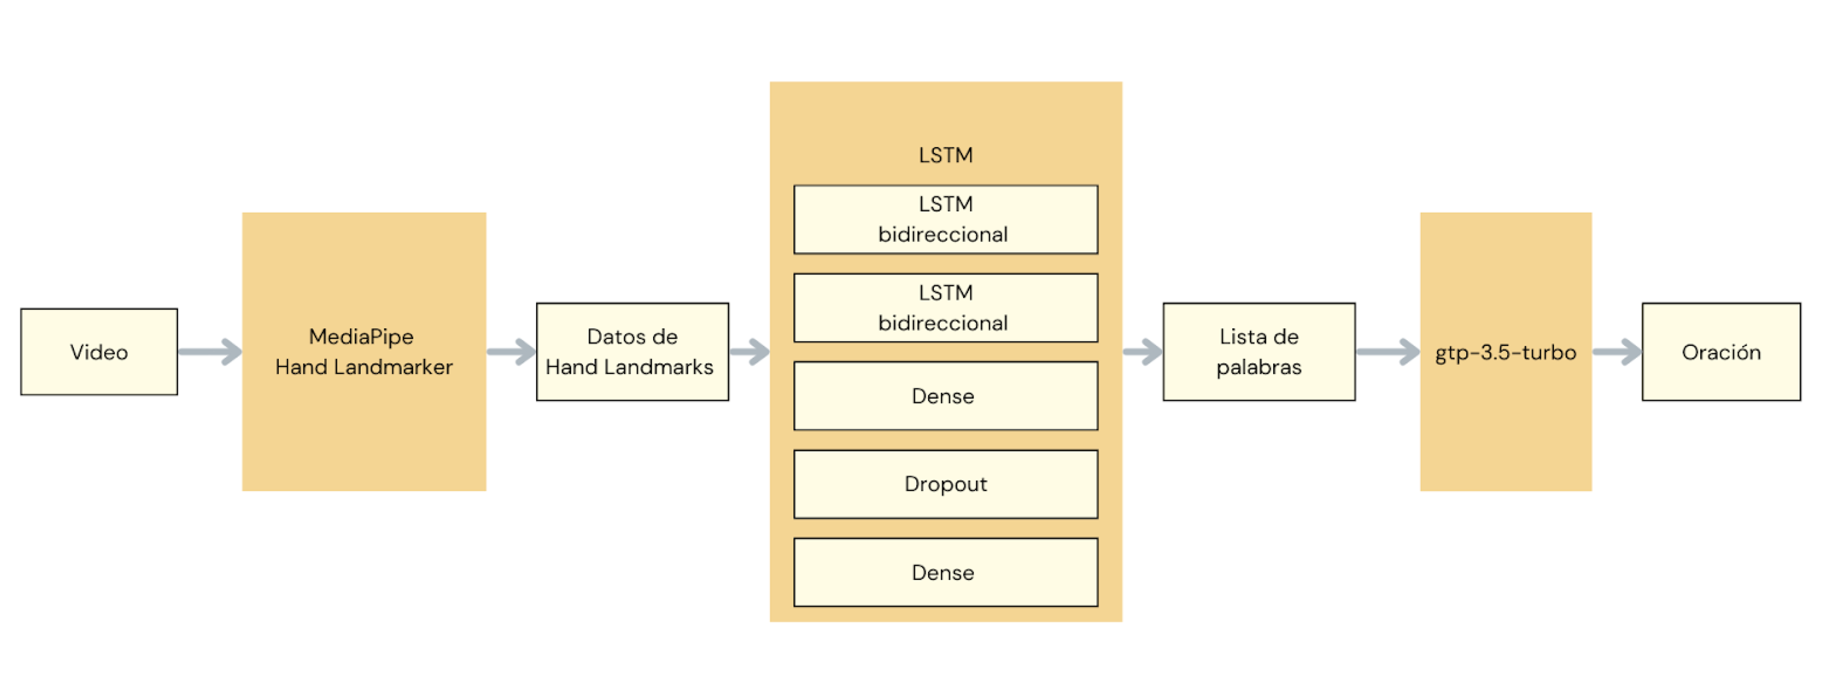
\includegraphics[width=5in]{figuras/architecture-diagram.png}
		\caption{Diagrama de bloques de la arquitectura propuesta}
		\label{fig1}
\end{figure}

\section{Experimentos}

En esta sección se describe el diseño y configuración de los experimentos realizados para validar la hipótesis.


\section{Resultados}

En esta sección se presentan los resultados para cada experimento.


\section{Conclusiones}

En el presente trabajo se ha realizado una revisión del estado del arte de los métodos para interpretar la Lengua de señas Chilena, así como otros métodos utilizados internacionalmente, proponiendo una solución que combina diferentes modelos para obtener un resultado con una tasa de acierto y porcentaje de coincidencia de las traducciones finales, sobre 90\%, en el contexto de una arquitectura cliente-servidor que permita su ejecución desde dispositivos portátiles, en particular de baja y media gama, con una latencia en el orden de los 1 a 2 segundos.


De estos resultados podemos concluir que este esquema tiene potencial para permitir la accesibilidad de las personas sordas a los servicios de salud, sin necesidad de un intérprete. Sin embargo, aún quedan grandes retos por resolver. Por un lado, es necesario recopilar un conjunto de datos robusto y representativo de la Lengua de Señas Chilena, ya que los datos actuales son muy limitados y no abarcan la diversidad de señas necesarias para aplicaciones generalizadas. Por otro lado, reducir la latencia a menos de un segundo, mejoraría significativamente la calidad de la comunicación, permitiendo interacciones más fluidas.


\begin{thebibliography}{99}

\bibitem{cita1}  Herrera, M. (2023, Febrero) Falta de inclusión, estigma social y discriminación: la compleja realidad diaria que vive una persona sorda en Chile. La Tercera. Santiago. p. 1 

\bibitem{cita2} Mendía R. y García C. (2021, Enero). Comunidad sorda y salud mental: Un abandono silencioso. La Tercera. Santiago. p. 1

\bibitem{cita3} Gonzalez, C. y Yimes F. (2016) Sistema de reconocimiento gestual de lengua de señas chilena mediante cámara digital p. 36-41

\bibitem{cita4} Acuña, X., Adamo, D. y Cabrera I. (2009) Diccionario Bilingüe de Lengua de Señas Chilena-Español. p. 17-18

\bibitem{cita5} Andrare, L. y Catril, R. (2022) Reconocimiento en tiempo real del alfabeto de lengua de señas chilena empleando aprendizaje automático. p. 53-62

\bibitem{cita6} Pathan, R. K., Biswas, M., Yasmin, S., Khandaker, M. U., Salman, M., \& Youssef, A. A. F. (2023). Sign language recognition using the fusion of image and hand landmarks through multi-headed convolutional neural network. p. 4-9

\bibitem{cita7}  Bala, D., Sarkar, B., Abdullah, M. I., \& Hossain, M. A. (2021). American Sign Language alphabets recognition using convolutional neural network. International Journal of Knowledge Based Computer Systems.

\bibitem{cita8}  Makkar, A., Makkar, D., Patel, A., \& Hebert, L. (2024). SignSpeak: Open-source time series classification for ASL translation.

\bibitem{cita9}  Renjith, S., \& Manazhy, R. (2024). Sign language: A systematic review on classification and recognition. P. 14-15

\bibitem{cita10} Gong, J., Foo, L. G., He, Y., Rahmani, H., \& Liu, J. (2024). LLMs are good sign language translators. 

\bibitem{cita11} Imran, A., Hulikal, M. S., \& Gardi, H. A. A. (2024). Real Time American Sign Language Detection Using YOLO-v9

\bibitem{cita12} Ministerio de Desarrollo Social y Servicio Nacional de la Discapacidad (SENADIS). (2015). II Estudio Nacional de la Discapacidad.


\end{thebibliography}

\end{document}
